\documentclass{beamer}
\usepackage[latin1]{inputenc}

\usetheme{Madrid}
\usecolortheme{default}
\usepackage{amsmath}
\usepackage{amssymb,amsfonts,amsthm}
\usepackage{txfonts}
\usepackage{tkz-euclide}
\usepackage{listings}
\usepackage{adjustbox}
\usepackage{array}
\usepackage{tabularx}
\usepackage{gvv}
\usepackage{lmodern}
\usepackage{circuitikz}
\usepackage{tikz}
\usepackage{graphicx}
\usepackage{gensymb}
\usepackage{physics}

\setbeamertemplate{page number in head/foot}[totalframenumber]

\usepackage{tcolorbox}
\tcbuselibrary{minted,breakable,xparse,skins}



\definecolor{bg}{gray}{0.95}
\DeclareTCBListing{mintedbox}{O{}m!O{}}{%
  breakable=true,
  listing engine=minted,
  listing only,
  minted language=#2,
  minted style=default,
  minted options={%
    linenos,
    gobble=0,
    breaklines=true,
    breakafter=,,
    fontsize=\small,
    numbersep=8pt,
    #1},
  boxsep=0pt,
  left skip=0pt,
  right skip=0pt,
  left=25pt,
  right=0pt,
  top=3pt,
  bottom=3pt,
  arc=5pt,
  leftrule=0pt,
  rightrule=0pt,
  bottomrule=2pt,
  toprule=2pt,
  colback=bg,
  colframe=orange!70,
  enhanced,
  overlay={%
    \begin{tcbclipinterior}
    \fill[orange!20!white] (frame.south west) rectangle ([xshift=20pt]frame.north west);
    \end{tcbclipinterior}},
  #3,
}
\lstset{
    language=C,
    basicstyle=\ttfamily\small,
    keywordstyle=\color{blue},
    stringstyle=\color{orange},
    commentstyle=\color{green!60!black},
    numbers=left,
    numberstyle=\tiny\color{gray},
    breaklines=true,
    showstringspaces=false,
}
\title{4.13.30}
\date{19th september, 2025}
\author{Vishwambhar - EE25BTECH11025}

\begin{document}

\frame{\titlepage}
\begin{frame}{Question}
If $\vec{P}=(1,0)$, $\vec{Q} = (-1,0)$  and $\vec{R}=(2,0)$ are three given points, then the locus of point $\vec{S}$ satisfying the relation $(SQ)^2+(SR)^2=2(SP)^2$, is:\\
\begin{enumerate}
    \item a straight line parallel to $X$ axis
    \item a circle passing through the origin
    \item a circle with the center at the origin
    \item a straight line parallel to $Y$ axis
\end{enumerate}
\end{frame}

\begin{frame}{Given}
Given
\begin{align}
    \vec{P}=\myvec{1\\0}; \vec{Q}=\myvec{-1\\0}; \vec{R}=\myvec{2\\0}\\
    \vec{S}=\myvec{x\\y}
\end{align}
\end{frame}

\begin{frame}{Solving}
\begin{align}
    ||\vec{Q}-\vec{S}||^2+||\vec{R}-\vec{S}||^2=2||\vec{P}-\vec{S}||^2\\
    \myvec{\vec{Q}-\vec{S}}^\top\myvec{\vec{Q}-\vec{S}}+\myvec{\vec{R}-\vec{S}}^\top\myvec{\vec{R}-\vec{S}}=2\myvec{\vec{P}-\vec{S}}^\top\myvec{\vec{P}-\vec{S}}\\
    ||\vec{Q}||^2+||\vec{R}||^2-2||\vec{P}||^2=\vec{S}^\top+\vec{Q}^\top\vec{S}+\vec{S}^\top\vec{R}+\vec{R}^\top\vec{S}-2\vec{S}^\top\vec{P}-2\vec{P}^\top\vec{S}\\
    ||\vec{Q}||^2+||\vec{R}||^2-2||\vec{P}||^2=\vec{S}^\top\myvec{\vec{Q}+\vec{R}-2\vec{P}}+\vec{S}\myvec{\vec{Q}+\vec{R}-2\vec{P}}^\top\\
    ||\vec{Q}||^2+||\vec{R}||^2-2||\vec{P}||^2=2\myvec{\vec{Q}+\vec{R}-2\vec{P}}^\top\vec{S}
\end{align}
\end{frame}

\begin{frame}{Solving}
Equation (7) is of the form:
\begin{align}
    \vec{n}^\top\vec{x}=c
\end{align}
\begin{align}
    \myvec{\vec{Q}+\vec{R}-2\vec{P}}^\top\vec{S}= \frac{||\vec{Q}||^2+||\vec{R}||^2-2||\vec{P}||^2}{2}
\end{align}
\end{frame}

\begin{frame}{Substituting}
Substituting values:
\begin{align}
    \myvec{\myvec{-1\\0}+\myvec{2\\0}-2\myvec{1\\0}}^\top\vec{S}= \frac{\brak{\brak{-1}^2+0^2}+\brak{2^2+0^2}-2\brak{1^2+0^2}}{2}
\end{align}
\begin{align}
    \myvec{-1\\0}^\top\vec{S}=\frac{3}{2}
\end{align}

Hence the locus of $\vec{s}$ is a line parallel to $Y$-axis.
\end{frame}

\begin{frame}[fragile]
    \frametitle{C Code}
    \begin{lstlisting}
#include<stdio.h>
#include<math.h>
double arrP[2] = {1,0};
double arrQ[2] = {-1,0};
double arrR[2] = {2,0};

void give_data(double *points){
    double normal[2];
    for(int i = 0; i<2; i++){
        normal[i] = arrQ[i]+arrR[i]-(2*arrP[i]);
    }
    \end{lstlisting}
\end{frame}

\begin{frame}[fragile]
    \frametitle{C Code}
    \begin{lstlisting}
  double k=0;
    for(int i = 0; i<2; i++){
        k+=(pow(arrQ[i],2)+pow(arrR[i],2)-(2*pow(arrP[i],2)))/2;

    }
    points[0] = arrP[0]; points[1] = arrP[1];
    points[2] = arrQ[0]; points[3] = arrQ[1];
    points[4] = arrR[0]; points[5] = arrR[1];
    points[6] = normal[0]; points[7] = normal[1];
    points[8] = k;
}
 
    \end{lstlisting}
\end{frame}

\begin{frame}[fragile]
    \frametitle{Python Code 1}
    \begin{lstlisting}
import ctypes as ct

lib = ct.CDLL("./problem.so")

lib.give_data.argtypes = [ct.POINTER(ct.c_double)]

points = ct.c_double*9

data = points()

lib.give_data(data)

def send_data():
    return data
    \end{lstlisting}
\end{frame}

\begin{frame}[fragile]
    \frametitle{Python Code 2}
    \begin{lstlisting}
import matplotlib.pyplot as plt
import numpy as np
from call import send_data

data = send_data()

y = np.linspace(-5, 5, 100)
x = ((data[7]*y)+data[8])/data[6]

X = [data[0], data[2], data[4]]
Y = [data[1], data[3], data[5]]

plt.plot(x, y, '-r')
plt.plot(X, Y, 'ko')
    \end{lstlisting}
\end{frame}

\begin{frame}[fragile]
    \frametitle{Python Code 2}
    \begin{lstlisting}
plt.text(0.6, 0.1, "(1,0)", fontsize=10, color="black")
plt.text(-1.1, 0.1, "(-1,0)", fontsize=10, color="black")
plt.text(2.1, 0.1, "(2,0)", fontsize=10, color="black")
plt.text(-1.51, 3.20, r"$x=\frac{3}{2}$", fontsize=13, color="black")

plt.axvline(x=0, color='k', linewidth=1.5)
plt.axhline(y=0, color='k', linewidth=1.5)

plt.xlabel("X-axis")
plt.ylabel("Y-axis")
plt.grid(True)
plt.axis("equal")
plt.savefig("../figs/plot.png")
plt.show()  \end{lstlisting}
\end{frame}

\begin{frame}{Plot}
    \begin{figure}
        \centering
        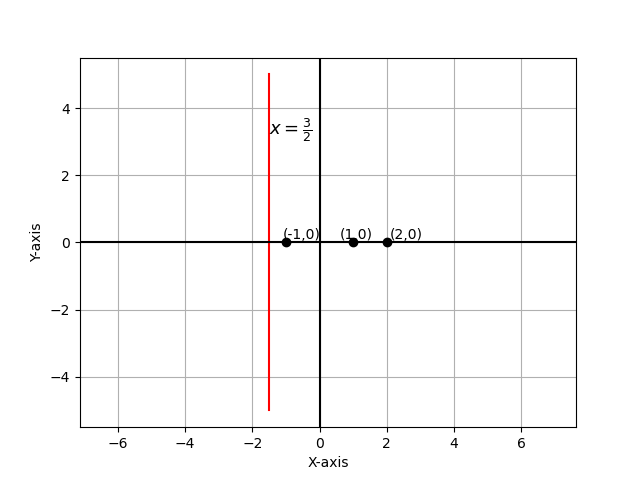
\includegraphics[width=0.5\columnwidth]{../figs/plot.png}
        \caption{Plot of the given points and locus of $\vec{S}$}
        \label{fig:fig}
    \end{figure}
\end{frame}
\end{document}
